\documentclass[12pt,twoside]{article}

\newcommand{\reporttitle}{Project 3: Traffic Signs Classifier}
\newcommand{\reportauthor}{Thomas Teh}
\newcommand{\reporttype}{Project Report}
\newcommand{\cid}{0124 3008}

% include files that load packages and define macros
%%%%%%%%%%%%%%%%%%%%%%%%%%%%%%%%%%%%%%%%%
% University Assignment Title Page 
% LaTeX Template
% Version 1.0 (27/12/12)
%
% This template has been downloaded from:
% http://www.LaTeXTemplates.com
%
% Original author:
% WikiBooks (http://en.wikibooks.org/wiki/LaTeX/Title_Creation)
%
% License:
% CC BY-NC-SA 3.0 (http://creativecommons.org/licenses/by-nc-sa/3.0/)
% 
% Instructions for using this template:
% This title page is capable of being compiled as is. This is not useful for 
% including it in another document. To do this, you have two options: 
%
% 1) Copy/paste everything between \begin{document} and \end{document} 
% starting at \begin{titlepage} and paste this into another LaTeX file where you 
% want your title page.
% OR
% 2) Remove everything outside the \begin{titlepage} and \end{titlepage} and 
% move this file to the same directory as the LaTeX file you wish to add it to. 
% Then add \input{./title_page_1.tex} to your LaTeX file where you want your
% title page.
%
%----------------------------------------------------------------------------------------
%	PACKAGES AND OTHER DOCUMENT CONFIGURATIONS
%----------------------------------------------------------------------------------------
\usepackage{ifxetex}
\usepackage{textpos}
%\usepackage{natbib}
%\usepackage{breqn}
\usepackage{kpfonts}
\usepackage[a4paper,hmargin=2.8cm,vmargin=2.0cm,includeheadfoot]{geometry}
\usepackage{ifxetex}
\usepackage{stackengine}
\usepackage{tabularx,longtable,multirow,subfigure,caption}%hangcaption
\usepackage{fncylab} %formatting of labels
\usepackage{fancyhdr}
\usepackage{color}
\usepackage[tight,ugly]{units}
\usepackage{url}
\usepackage{float}
\usepackage[english]{babel}
\usepackage{amsmath}
\usepackage{graphicx}
\usepackage[colorinlistoftodos]{todonotes}
\usepackage{dsfont}
\usepackage{epstopdf} % automatically replace .eps with .pdf in graphics
\usepackage{natbib}
\usepackage{backref}
\usepackage{array}
\usepackage{latexsym}
\usepackage{etoolbox}
\usepackage{algorithmic}
\usepackage[]{algorithm2e}

\usepackage{enumerate} % for numbering with [a)] format 



\ifxetex
\usepackage{fontspec}
\setmainfont[Scale=.8]{OpenDyslexic-Regular}
\else
\usepackage[pdftex,pagebackref,hypertexnames=false,colorlinks]{hyperref} % provide links in pdf
\hypersetup{pdftitle={},
  pdfsubject={}, 
  pdfauthor={\reportauthor},
  pdfkeywords={}, 
  pdfstartview=FitH,
  pdfpagemode={UseOutlines},% None, FullScreen, UseOutlines
  bookmarksnumbered=true, bookmarksopen=true, colorlinks,
    citecolor=black,%
    filecolor=black,%
    linkcolor=black,%
    urlcolor=black}
\usepackage[all]{hypcap}
\fi

\usepackage{tcolorbox}
\usepackage{hyperref}
% various theorems
\usepackage{ntheorem}
\theoremstyle{break}
\newtheorem{lemma}{Lemma}
\newtheorem{theorem}{Theorem}
\newtheorem{remark}{Remark}
\newtheorem{definition}{Definition}
\newtheorem{proof}{Proof}

% example-environment
\newenvironment{example}[1][]
{ 
\vspace{4mm}
\noindent\makebox[\linewidth]{\rule{\hsize}{1.5pt}}
\textbf{Example #1}\\
}
{ 
\noindent\newline\makebox[\linewidth]{\rule{\hsize}{1.0pt}}
}



%\renewcommand{\rmdefault}{pplx} % Palatino
% \renewcommand{\rmdefault}{put} % Utopia

\ifxetex
\else
\renewcommand*{\rmdefault}{bch} % Charter
\renewcommand*{\ttdefault}{cmtt} % Computer Modern Typewriter
%\renewcommand*{\rmdefault}{phv} % Helvetica
%\renewcommand*{\rmdefault}{iwona} % Avant Garde
\fi

\setlength{\parindent}{0em}  % indentation of paragraph

\setlength{\headheight}{14.5pt}
\pagestyle{fancy}
\fancyfoot[ER,OL]{\thepage}%Page no. in the left on
                                %odd pages and on right on even pages
\fancyfoot[OC,EC]{\sffamily }
\renewcommand{\headrulewidth}{0.1pt}
\renewcommand{\footrulewidth}{0.1pt}
\captionsetup{margin=10pt,font=small,labelfont=bf}


%--- chapter heading

\def\@makechapterhead#1{%
  \vspace*{10\p@}%
  {\parindent \z@ \raggedright %\sffamily
        %{\Large \MakeUppercase{\@chapapp} \space \thechapter}
        %\\
        %\hrulefill
        %\par\nobreak
        %\vskip 10\p@
    \interlinepenalty\@M
    \Huge \bfseries 
    \thechapter \space\space #1\par\nobreak
    \vskip 30\p@
  }}

%---chapter heading for \chapter*  
\def\@makeschapterhead#1{%
  \vspace*{10\p@}%
  {\parindent \z@ \raggedright
    \sffamily
    \interlinepenalty\@M
    \Huge \bfseries  
    #1\par\nobreak
    \vskip 30\p@
  }}
  



% %%%%%%%%%%%%% boxit
\def\Beginboxit
   {\par
    \vbox\bgroup
	   \hrule
	   \hbox\bgroup
		  \vrule \kern1.2pt %
		  \vbox\bgroup\kern1.2pt
   }

\def\Endboxit{%
			      \kern1.2pt
		       \egroup
		  \kern1.2pt\vrule
		\egroup
	   \hrule
	 \egroup
   }	

\newenvironment{boxit}{\Beginboxit}{\Endboxit}
\newenvironment{boxit*}{\Beginboxit\hbox to\hsize{}}{\Endboxit}



\allowdisplaybreaks

\makeatletter
\newcounter{elimination@steps}
\newcolumntype{R}[1]{>{\raggedleft\arraybackslash$}p{#1}<{$}}
\def\elimination@num@rights{}
\def\elimination@num@variables{}
\def\elimination@col@width{}
\newenvironment{elimination}[4][0]
{
    \setcounter{elimination@steps}{0}
    \def\elimination@num@rights{#1}
    \def\elimination@num@variables{#2}
    \def\elimination@col@width{#3}
    \renewcommand{\arraystretch}{#4}
    \start@align\@ne\st@rredtrue\m@ne
}
{
    \endalign
    \ignorespacesafterend
}
\newcommand{\eliminationstep}[2]
{
    \ifnum\value{elimination@steps}>0\leadsto\quad\fi
    \left[
        \ifnum\elimination@num@rights>0
            \begin{array}
            {@{}*{\elimination@num@variables}{R{\elimination@col@width}}
            |@{}*{\elimination@num@rights}{R{\elimination@col@width}}}
        \else
            \begin{array}
            {@{}*{\elimination@num@variables}{R{\elimination@col@width}}}
        \fi
            #1
        \end{array}
    \right]
    & 
    \begin{array}{l}
        #2
    \end{array}
    &%                                    moved second & here
    \addtocounter{elimination@steps}{1}
}
\makeatother

%% Fast macro for column vectors
\makeatletter  
\def\colvec#1{\expandafter\colvec@i#1,,,,,,,,,\@nil}
\def\colvec@i#1,#2,#3,#4,#5,#6,#7,#8,#9\@nil{% 
  \ifx$#2$ \begin{bmatrix}#1\end{bmatrix} \else
    \ifx$#3$ \begin{bmatrix}#1\\#2\end{bmatrix} \else
      \ifx$#4$ \begin{bmatrix}#1\\#2\\#3\end{bmatrix}\else
        \ifx$#5$ \begin{bmatrix}#1\\#2\\#3\\#4\end{bmatrix}\else
          \ifx$#6$ \begin{bmatrix}#1\\#2\\#3\\#4\\#5\end{bmatrix}\else
            \ifx$#7$ \begin{bmatrix}#1\\#2\\#3\\#4\\#5\\#6\end{bmatrix}\else
              \ifx$#8$ \begin{bmatrix}#1\\#2\\#3\\#4\\#5\\#6\\#7\end{bmatrix}\else
                 \PackageError{Column Vector}{The vector you tried to write is too big, use bmatrix instead}{Try using the bmatrix environment}
              \fi
            \fi
          \fi
        \fi
      \fi
    \fi
  \fi 
}  
\makeatother

\robustify{\colvec}

%%% Local Variables: 
%%% mode: latex
%%% TeX-master: "notes"
%%% End: 
 % various packages needed for maths etc.
% quick way of adding a figure
\newcommand{\fig}[3]{
 \begin{center}
 \scalebox{#3}{\includegraphics[#2]{#1}}
 \end{center}
}

%\newcommand*{\point}[1]{\vec{\mkern0mu#1}}
\newcommand{\ci}[0]{\perp\!\!\!\!\!\perp} % conditional independence
\newcommand{\point}[1]{{#1}} % points 
\renewcommand{\vec}[1]{{\boldsymbol{{#1}}}} % vector
\newcommand{\mat}[1]{{\boldsymbol{{#1}}}} % matrix
\newcommand{\R}[0]{\mathds{R}} % real numbers
\newcommand{\Z}[0]{\mathds{Z}} % integers
\newcommand{\N}[0]{\mathds{N}} % natural numbers
\newcommand{\nat}[0]{\mathds{N}} % natural numbers
\newcommand{\Q}[0]{\mathds{Q}} % rational numbers
\ifxetex
\newcommand{\C}[0]{\mathds{C}} % complex numbers
\else
\newcommand{\C}[0]{\mathds{C}} % complex numbers
\fi
\newcommand{\tr}[0]{\text{tr}} % trace
\renewcommand{\d}[0]{\mathrm{d}} % total derivative
\newcommand{\inv}{^{-1}} % inverse
\newcommand{\id}{\mathrm{id}} % identity mapping
\renewcommand{\dim}{\mathrm{dim}} % dimension
\newcommand{\rank}[0]{\mathrm{rk}} % rank
\newcommand{\determ}[1]{\mathrm{det}(#1)} % determinant
\newcommand{\scp}[2]{\langle #1 , #2 \rangle}
\newcommand{\kernel}[0]{\mathrm{ker}} % kernel/nullspace
\newcommand{\img}[0]{\mathrm{Im}} % image
\newcommand{\idx}[1]{{(#1)}}
\DeclareMathOperator*{\diag}{diag}
\newcommand{\E}{\mathds{E}} % expectation
\newcommand{\var}{\mathds{V}} % variance
\newcommand{\gauss}[2]{\mathcal{N}\big(#1,\,#2\big)} % gaussian distribution N(.,.)
\newcommand{\gaussx}[3]{\mathcal{N}\big(#1\,|\,#2,\,#3\big)} % gaussian distribution N(.|.,.)
\newcommand{\gaussBig}[2]{\mathcal{N}\left(#1,\,#2\right)} % see above, but with brackets that adjust to the height of the arguments
\newcommand{\gaussxBig}[3]{\mathcal{N}\left(#1\,|\,#2,\,#3\right)} % see above, but with brackets that adjust to the height of the arguments
\DeclareMathOperator{\cov}{Cov} % covariance (matrix) 
\ifxetex
\renewcommand{\T}[0]{^\top} % transpose
\else
\newcommand{\T}[0]{^\top}
\fi
% matrix determinant
\newcommand{\matdet}[1]{
\left|
\begin{matrix}
#1
\end{matrix}
\right|
}



%%% various color definitions
\definecolor{darkgreen}{rgb}{0,0.6,0}

\newcommand{\blue}[1]{{\color{blue}#1}}
\newcommand{\red}[1]{{\color{red}#1}}
\newcommand{\green}[1]{{\color{darkgreen}#1}}
\newcommand{\orange}[1]{{\color{orange}#1}}
\newcommand{\magenta}[1]{{\color{magenta}#1}}
\newcommand{\cyan}[1]{{\color{cyan}#1}}


% redefine emph
\renewcommand{\emph}[1]{\blue{\bf{#1}}}

% place a colored box around a character
\gdef\colchar#1#2{%
  \tikz[baseline]{%
  \node[anchor=base,inner sep=2pt,outer sep=0pt,fill = #2!20] {#1};
    }%
}%
 % short-hand notation and macros
\DontPrintSemicolon

%%%%%%%%%%%%%%%%%%%%%%%%%%%%

\begin{document}
% front page
% Last modification: 2016-09-29 (Marc Deisenroth)
\begin{titlepage}

\newcommand{\HRule}{\rule{\linewidth}{0.5mm}} % Defines a new command for the horizontal lines, change thickness here


%----------------------------------------------------------------------------------------
%	LOGO SECTION
%----------------------------------------------------------------------------------------

%
\includegraphics[width = 4cm]{./figures/imperial}\\[0.5cm] 

\begin{center} % Center remainder of the page

%----------------------------------------------------------------------------------------
%	HEADING SECTIONS
%----------------------------------------------------------------------------------------
\textsc{\LARGE \reporttype}\\[1.5cm] 
\textsc{\Large Udacity}\\[0.5cm] 
\textsc{\large Self-Driving Car Nanodegree}\\[0.5cm] 
%----------------------------------------------------------------------------------------
%	TITLE SECTION
%----------------------------------------------------------------------------------------

\HRule \\[0.4cm]
{ \huge \bfseries \reporttitle}\\ % Title of your document
\HRule \\[1.5cm]
\end{center}
%----------------------------------------------------------------------------------------
%	AUTHOR SECTION
%----------------------------------------------------------------------------------------

%\begin{minipage}{0.4\hsize}
\begin{flushleft} \large
\textsc{Author:}\\
\reportauthor~%(CID: \cid) % Your name
\end{flushleft}
\vspace{2cm}
\makeatletter
Date: \@date 

\vfill % Fill the rest of the page with whitespace



\makeatother


\end{titlepage}




%%%%%%%%%%%%%%%%%%%%%%%%%%%% Main document
\section{Introduction}
This project is part of the Self-Driving Car Nanodegree by Udacity and its objective is to train a traffic signs classifier. The data set used to train the model is the  German Traffic Sign Dataset and the summary of the data is given below:

\begin{center}
\begin{tabular}{|c|c|c|c|}
\hline
\textbf{Type}	& \textbf{Amount}		& \textbf{Image Size}			& \textbf{Color}\\\hline
Training			& 34799					&			$32\times32$			& RGB\\
Validation			& 4410						&			$32\times32$			& RGB\\
Test					& 12630 					&			$32\times32$			& RGB\\\hline
\end{tabular}
\end{center}

The dataset contains 43 different classes and samples of the training images are shown in Figure \ref{fig:sample}. Also, we visualize the distribution of the different classes and we can observe that there is a significant class imbalance as in Figure \ref{fig:image distribution}.

\begin{figure}[H]
	\begin{center}
		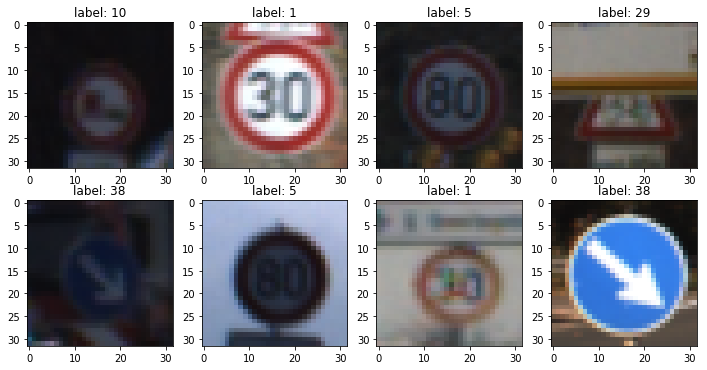
\includegraphics[width = 1.0\hsize]{./figures/Training_data.png} 
		\caption{Sample training images.} % caption of the figure
		\label{fig:sample} % a label. When we refer to this label from the text, the figure %number is included automatically
	\end{center}
\end{figure}


\begin{figure}[H]
	\begin{center}
		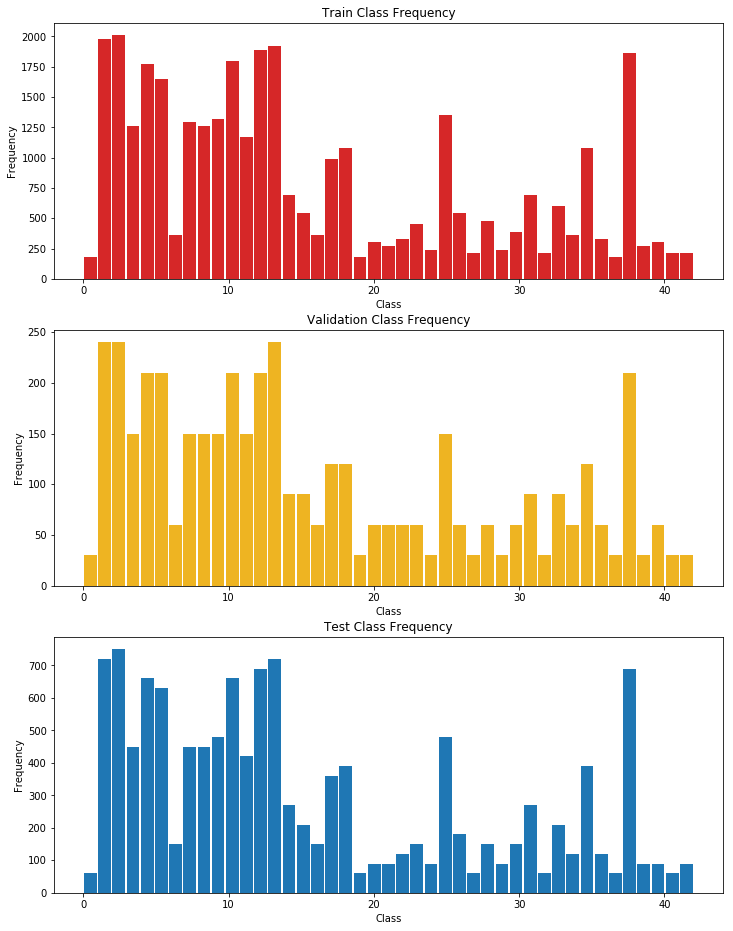
\includegraphics[width = 1.0\hsize]{./figures/Distribution.png} 
		\caption{\emph{Top: }Training Set \emph{Middle: }Validation \emph{Bottom: }Test} % caption of the figure
		\label{fig:image distribution} % a label. When we refer to this label from the text, the figure %number is included automatically
	\end{center}
\end{figure}

\newpage

\section{Image Preprocessing}
Preprocessing is done in the following steps:
\begin{enumerate}
	\item \textbf{Data Augmentation:} We augment the data by random performing the below transformations on the original training data set:
		\begin{itemize}
			\item Rotation: 25 degrees
			\item Width shift: 0.20
			\item Height shift: 0.20
			\item Zoom range: (0.80, 1.20)
		\end{itemize}
	With the augmentation, the amount of the training data available is tripled to 104,397.
	\item \textbf{Convert to Grayscale:} Since the colors of the signs do not make a big difference in terms of distinguishing the them, we convert the RGB images into grayscale. The advantage of this is it reduces computation, hence allow us to use a much deeper model without having to do distributed training on the data set.
	\item \textbf{Histogram Normalization:} I applied the Contrast Limite Adaptive Histogram Equalization (CLAHE) to make the edges of the signs more obvious.
\end{enumerate}

A sample of an image after preprocessing is shown in Figure \ref{fig:preprocessing}
\begin{figure}[H]
	\begin{center}
		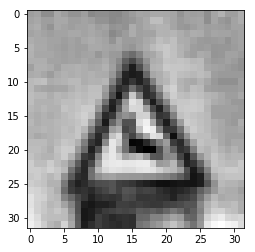
\includegraphics[width = 0.4\hsize]{./figures/Preprocessing.png} 
		\caption{Image after preprocessing} % caption of the figure
		\label{fig:preprocessing} % a label. When we refer to this label from the text, the figure %number is included automatically
	\end{center}
\end{figure}

\newpage

\section{Architecture and Hyperparameters}
The architecture that I used is shown below:

\begin{center}
\begin{tabular}{|c|}
\hline
\textbf{Input} \\\hline
\textbf{Convolution Layer} \\
Kernel size: $5\times 5$, N Kernels: 256 \\\hline
ReLU Activation Layer \\\hline
Max Pooling Layer \\
Kernel size: $2\times 2$\\\hline
\textbf{Convolution Layer} \\
Kernel size: $5\times 5$, N Kernels: 512 \\\hline
ReLU Activation Layer \\\hline
Max Pooling Layer \\\hline
Kernel size: $2\times 2$\\\hline
\textbf{Convolution Layer} \\
Kernel size: $5\times 5$, N Kernels: 2048 \\\hline
ReLU Activation Layer \\\hline
Max Pooling Layer \\
Kernel size: $2\times 2$\\\hline
\textbf{Dense Layer:} 1024 units \\\hline
ReLU Activation Layer \\\hline
Drop Out Layer: dropout prob = 0.60 \\\hline
\textbf{Dense Layer:} 512 units \\\hline
ReLU Activation Layer \\\hline
Drop Out Layer: dropout prob = 0.60 \\\hline
\textbf{Dense Layer:} 43 units \\\hline
\end{tabular}
\end{center}

The model is trained with ADAM optimization algorithm with the following hyperparameters:

\begin{center}
\begin{tabular}{|c|c|}
\hline
Hyperparameters		& 		Values\\\hline
Epoch						&		20\\
Batch Size				&		128\\
Learning Rate			&		0.0010\\\hline
\end{tabular}
\end{center}

Other comments:
\begin{itemize}
	\item Batch normalization did not help in the training process significantly and it results in a much slower training process. Hence I did not implement batch normalization in the final model.
	\item ELU activation works but they did not perform as well as ReLUs. Therefore, I decided to stick to ReLU activation unit.
	\item Drop out layers are used to prevent overfitting since we have a large number of neurons in the dense layers.
\end{itemize}

\newpage

\section{Performance}
The performance of the model after 20 epochs of training is shown in the table below:
\begin{center}
\begin{tabular}{|c|c|}
\hline
Data Type 		&		Accuracy \\\hline
Training			&		99.96\%\\
Validation			&		98.91\%\\
Test					&		98.20\%\\\hline
\end{tabular}
\end{center}

In addition to the test data, I sourced 6 images from the web and predictions from the model. The model achieves a 83.33\% accuracy. The model misclassified 1 image out of 6 images, and the reason is likely that this image contains a traffic sign that is vandalized (see Figure \ref{fig:vandalized_sign}).
\begin{figure}[H]
	\begin{center}
		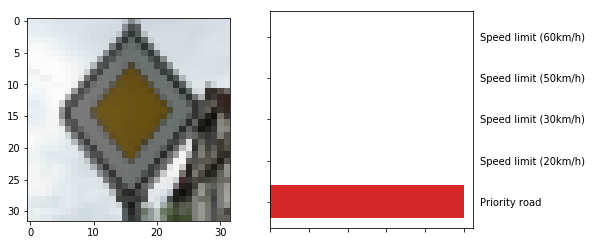
\includegraphics[width = 1.0\hsize]{./figures/Web1.png} 
		\caption{Image that was classified correctly.} % caption of the figure
		\label{fig:correct_classification} % a label. When we refer to this label from the text, the figure %number is included automatically
	\end{center}
\end{figure}


\begin{figure}[H]
	\begin{center}
		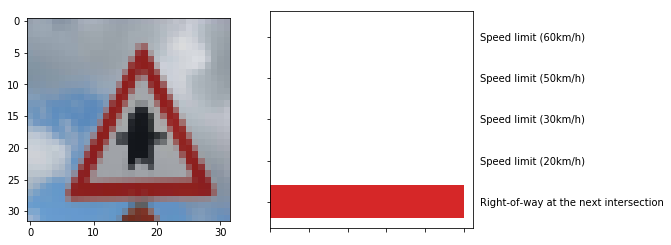
\includegraphics[width = 1.0\hsize]{./figures/Web2.png} 
		\caption{Image that was classified correctly.} % caption of the figure
		\label{fig:correct_classification} % a label. When we refer to this label from the text, the figure %number is included automatically
	\end{center}
\end{figure}


\begin{figure}[H]
	\begin{center}
		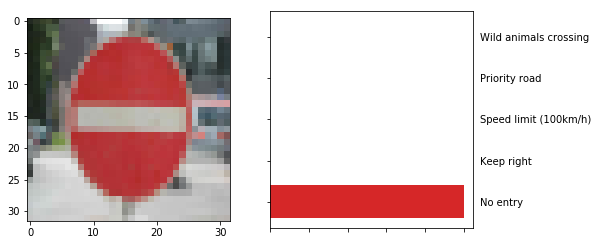
\includegraphics[width = 1.0\hsize]{./figures/Web3.png} 
		\caption{Image that was classified correctly.} % caption of the figure
		\label{fig:correct_classification} % a label. When we refer to this label from the text, the figure %number is included automatically
	\end{center}
\end{figure}



\begin{figure}[H]
	\begin{center}
		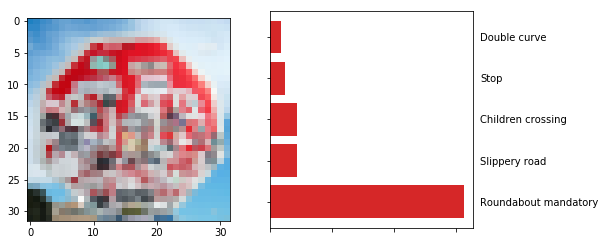
\includegraphics[width = 1.0\hsize]{./figures/Web4.png} 
		\caption{Image that was misclassified.} % caption of the figure
		\label{fig:vandalized_sign} % a label. When we refer to this label from the text, the figure %number is included automatically
	\end{center}
\end{figure}

\newpage

\section{Ideas for Improvements}
The following are some ideas for improving the project:
\begin{itemize}
	\item Can potentially do transfer learning. Instead of training a model from scratch, we can used a pretrained model such as ResNet or VGGNet. We can freeze the layers at the start of the model and only train the classifier. Given these models are trained on a larger data set, I would expect that the models developed using transfer learning to perform well.
	\item Adjust the training process to account for the class imbalance. This will improve the performance of the model.
	\item Expand the training data set by collecting the more data set. Most traffic signs in the German Traffic Signs data are similar or the same as those in other countries. We can potentially augment the data with real images of traffic signs from other countries.
\end{itemize}



%\bibliography{reference}
%\bibliographystyle{apalike}


\end{document}
%%% Local Variables: 
%%% mode: latex
%%% TeX-master: t
%%% End: 
